\documentclass[12pt,a4paper]{article}
\usepackage[utf8]{inputenc}
\usepackage[T2A]{fontenc}
\usepackage[russian]{babel}
\usepackage{graphicx}
\usepackage{geometry}
\geometry{margin=2cm}
\usepackage{booktabs}
\usepackage{amsmath}
\usepackage{float}
\usepackage{hyperref}
\hypersetup{
    colorlinks=true,
    linkcolor=blue,
    citecolor=blue,
    urlcolor=blue
}
\graphicspath{{images/}}

%--- Определение \addAuthor, если не задано -------------------------------
\providecommand{\addAuthor}[3]{%
  \par\textbf{#1}\\#2%
  \if\relax\detokenize{#3}\relax\else\\\texttt{#3}\fi%
  \vspace{0.5em}%
}
%-------------------------------------------------------------------------

\begin{document}

\begin{titlepage}
    \centering
    \vspace*{4cm}
    {\LARGE \textbf{Методы машинного обучения для анализа переменных звёзд}\\[0.5cm]}
    {\Large Отчёт о выполнении первых этапов проекта}\\[1cm]

    % Авторы
    \addAuthor{Бакакин Валерий Дмитриевич}{НИЯУ МИФИ}{val-bakakin@yandex.ru}

    \addAuthor{Жмелев Глеб Евгеньевич}{НИЯУ МИФИ}{}

    \addAuthor{Донецков Андрей Дмитриевич}{НИЯУ МИФИ}{}

    \vfill
    {\large \today}
\end{titlepage}

\tableofcontents
\newpage

\section{Введение}
Переменные звёзды играют важную роль в астрофизике, поскольку позволяют калибровать космологические расстояния и изучать процессы взаимодействия в двойных системах.
Рост объёмов астрономических данных, порождаемых массовыми обзорами (Gaia, Pan‑STARRS, CRTS и др.), делает необходимыми автоматические методы классификации астрономических объектов.
В настоящей работе применяются алгоритмы машинного обучения для решения двух подзадач:
\begin{enumerate}
    \item \textbf{Бинарная классификация}: отделение переменных звёзд от непеременных (Задание~1);
    \item \textbf{Многоклассовая классификация}: распределение переменных звёзд по шести основным типам (Задание~2).
\end{enumerate}
Отчёт покрывает только первые два этапа исследования на основе ноутбуков \texttt{task1.ipynb} и \texttt{task2.ipynb}, в которых выполнены подготовка данных, обучение моделей и оценка качества.

\section{Постановка задачи}
Формулировка исходных заданий приведена в приложенном документе~\cite{karachurin2025}.
Кратко цели этапов можно изложить так:
\begin{description}
    \item[Этап~1.] Построить алгоритм, способный с высокой точностью (целевой показатель $>$90~\%) отделять переменные звёзды от непеременных объектов.
    \item[Этап~2.] На основе выборки VSX обучить модель, классифицирующую объекты по шести типам (Cepheids, Delta~Scuti~etc., Eclipsing, Long~Period, Rotational, RR~Lyrae).
\end{description}
Обе задачи характеризуются сильно несбалансированными выборками, что обуславливает использование техники взвешивания классов и специальных метрик.

\section{Исходные данные и предварительная обработка}\label{sec:data}
\subsection{Состав датасета для бинарной классификации}
Для Этапа~1 подготовлен датасет \texttt{whole\_data\_practive3.csv} ($\approx60\,000$ записей, $34$ признака). 
Первичный анализ выявил сильную корреляцию между фотометрическими величинами (рис.~\ref{fig:corr}). 
Низкоинформативные признаки были удалены либо агрегированы.

\begin{figure}[H]
    \centering
    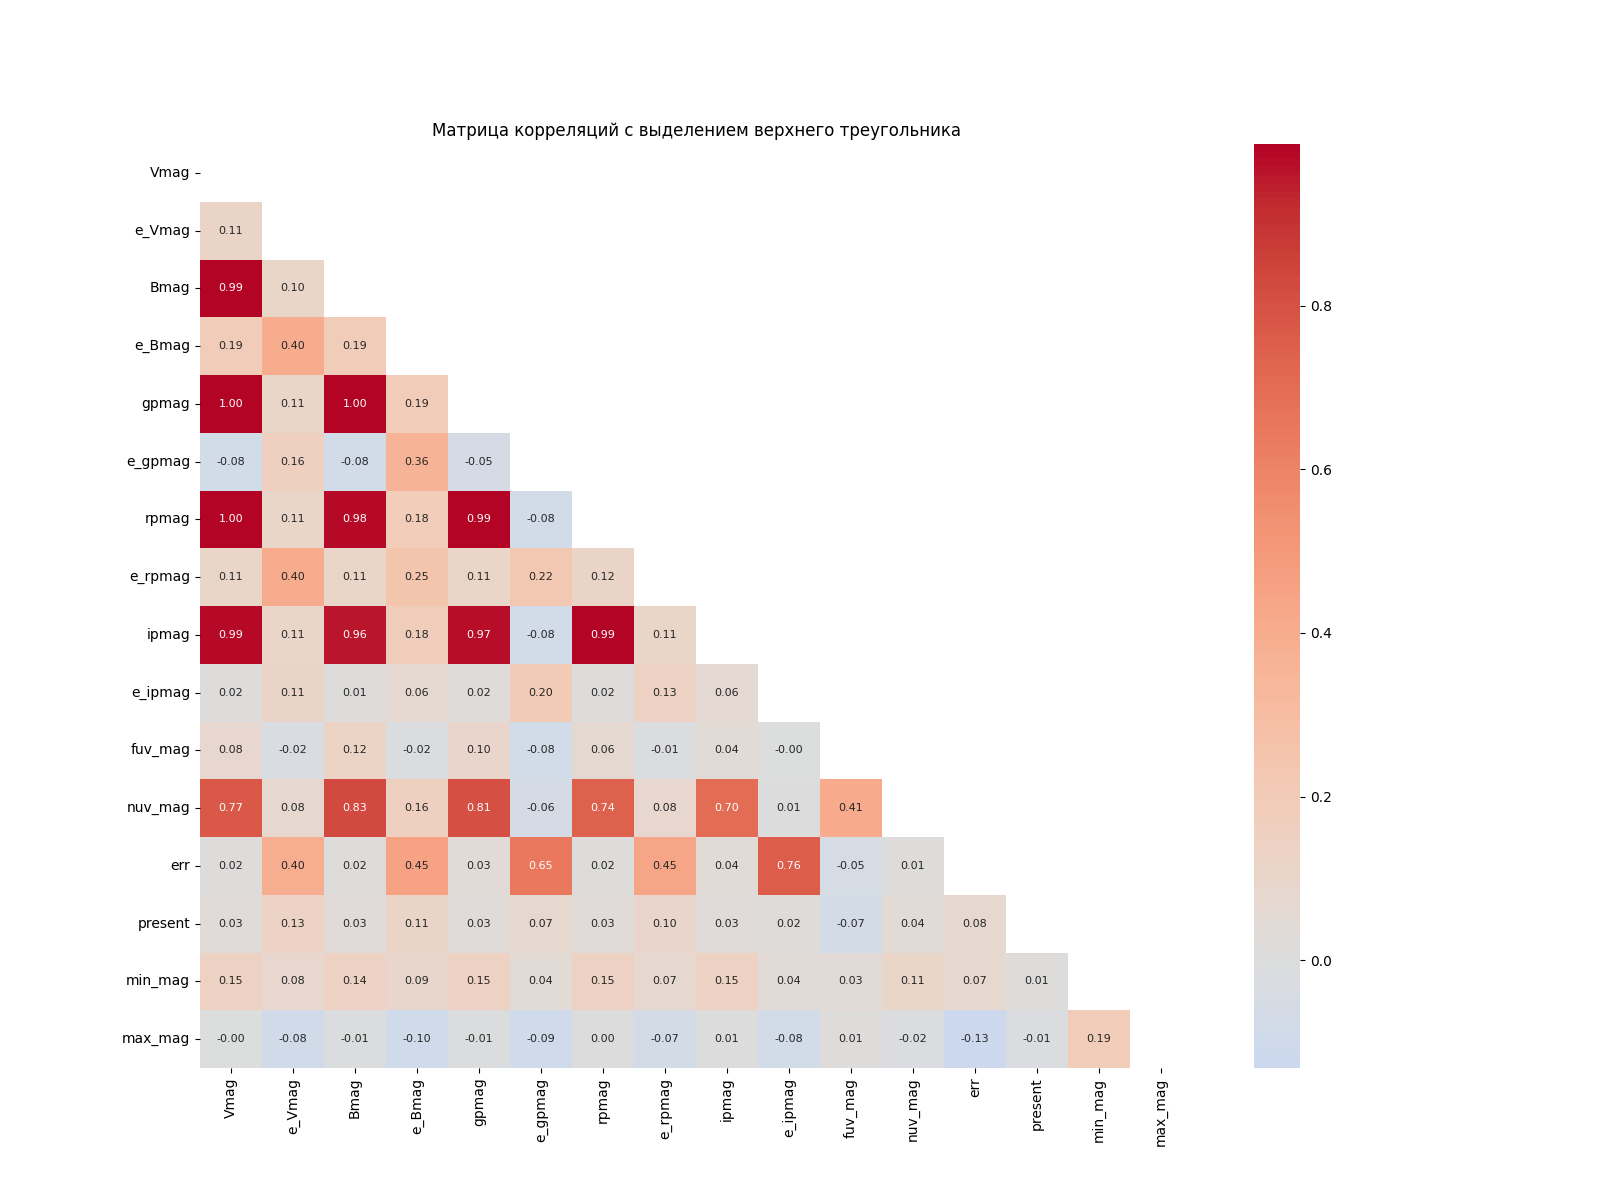
\includegraphics[width=\linewidth]{correlation_matrix.png}
    \caption{Матрица корреляций исходных признаков (фрагмент).}
    \label{fig:corr}
\end{figure}

\subsection{Обработка дисбаланса классов}
Распределение целевого признака \texttt{present} показано на рис.~\ref{fig:class_before}. 
Для коррекции дисбаланса использовано взвешивание классов в функции потерь \emph{для обеих} моделей; для оценки применялись метрики \texttt{ROC‑AUC} и F1 вместо простой accuracy.

\begin{figure}[H]
    \centering
    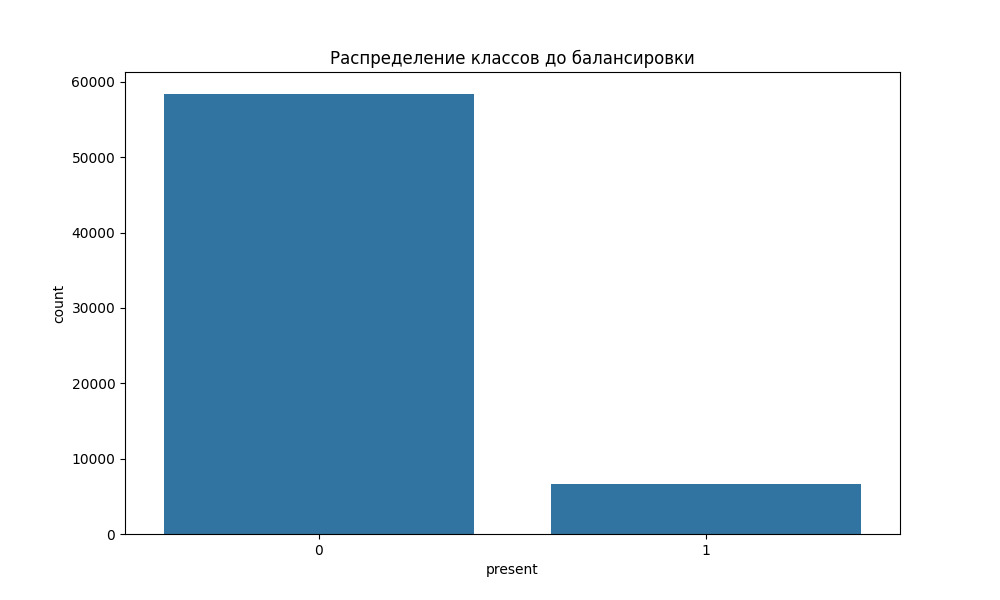
\includegraphics[width=.7\linewidth]{class_distribution_before.png}
    \caption{Распределение классов до балансировки.}
    \label{fig:class_before}
\end{figure}

\section{Бинарная классификация (Этап~1)}
\subsection{Методы}
Рассмотрены два алгоритма:
\begin{enumerate}
    \item \textbf{Градиентный бустинг} (GradientBoostingClassifier, 500 деревьев, learning\_rate=0.05, class\_weight).
    \item \textbf{Случайный лес} (RandomForestClassifier, 800 деревьев, max\_features=\texttt{sqrt}, class\_weight).
\end{enumerate}
Отбор гиперпараметров проводился сеточным поиском с 5‑кратной стратифицированной кросс‑валидацией.

\subsection{Результаты}
Сводные метрики приведены в табл.~\ref{tab:bin-metrics}. Случайный лес демонстрирует лучшие показатели (accuracy~=~0.94, F1~=~0.72).

\begin{table}[H]
    \centering
    \caption{Метрики бинарных моделей на тестовой выборке}
    \label{tab:bin-metrics}
    \begin{tabular}{lcccc}
        \toprule
        \textbf{Алгоритм} & \textbf{Accuracy} & \textbf{Precision} & \textbf{Recall} & \textbf{F1}\\
        \midrule
        Градиентный бустинг & 0.856 & 0.389 & 0.800 & 0.523\\
        Случайный лес       & 0.939 & 0.655 & 0.799 & 0.720\\
        \bottomrule
    \end{tabular}
\end{table}

\begin{figure}[H]
    \centering
    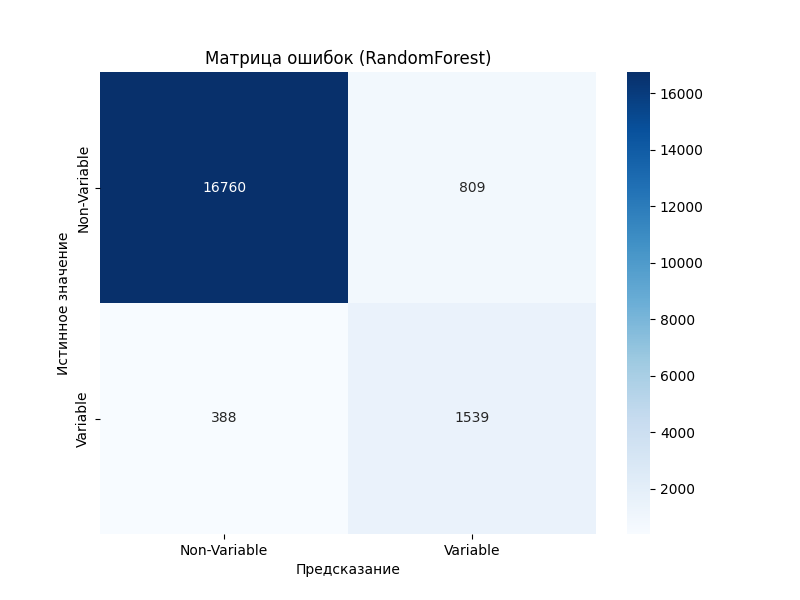
\includegraphics[width=.6\linewidth]{confusion_matrix_RandomForest.png}
    \caption{Confusion matrix: Random Forest.}
    \label{fig:cm-rf}
\end{figure}

\section{Многоклассовая классификация (Этап~2)}
\subsection{Подготовка выборки}
Каталог AAVSO VSX был загружен через \texttt{astroquery} (см. модуль \texttt{modules.py}) и преобразован в таблицу Parquet размера $\approx124\,000$ объектов.
Для уменьшения дисбаланса редкие классы были объединены, в результате оставлены шесть наиболее многочисленных типов.

\begin{figure}[H]
    \centering
    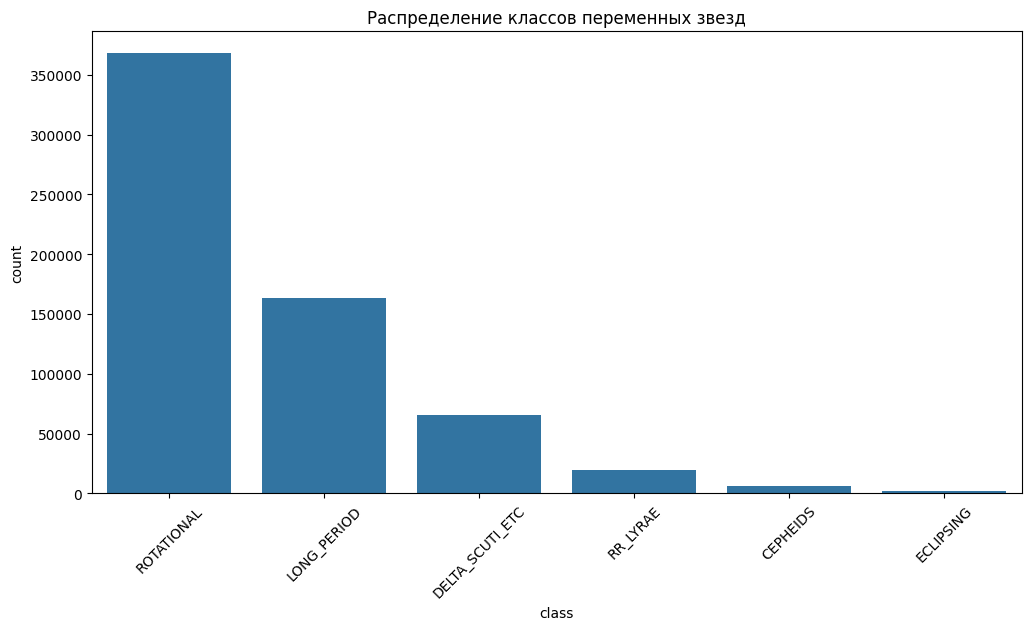
\includegraphics[width=.7\linewidth]{class_distribution_multiclass.png}
    \caption{Распределение классов в мультиклассовой задаче.}
    \label{fig:multiclass-dist}
\end{figure}

\subsection{Модель}
В качестве базовой модели выбран \textbf{полносвязный нейронный классификатор}:
\begin{itemize}
    \item Архитектура: 3 скрытых слоя (512, 256, 128 нейронов), активация ReLU.
    \item Регуляризация: Dropout 0.3, BatchNormalization.
    \item Оптимизатор: Adam, learning rate $10^{-3}$, class\_weights.
    \item Обучение: 50 эпох, early stopping по валидационному F1.
\end{itemize}
Для категориальных признаков применён \texttt{SMOTENC} с целью синтеза миноритарных примеров.

\subsection{Качество классификации}
Сводный отчёт модели приведён в табл.~\ref{tab:class-report}. 
Достигнута общая точность 0.95, однако F1 класса \texttt{ECLIPSING} остаётся низким (0.19) из-за крайне малой представленности в трейне.

\begin{table}[H]
    \centering
    \caption{Классификационный отчёт мультиклассовой модели}
    \label{tab:class-report}
    \begin{tabular}{lcccc}
        \toprule
        \textbf{Класс} & \textbf{Precision} & \textbf{Recall} & \textbf{F1} & \textbf{Support}\\\midrule
        CEPHEIDS & 0.64 & 0.85 & 0.73 & 1\,289\\
        DELTA\_SCUTI\_ETC & 0.85 & 0.93 & 0.89 & 13\,069\\
        ECLIPSING & 0.11 & 0.88 & 0.19 & 378\\
        LONG\_PERIOD & 1.00 & 1.00 & 1.00 & 32\,632\\
        ROTATIONAL & 1.00 & 0.93 & 0.96 & 73\,577\\
        RR\_LYRAE & 0.86 & 0.97 & 0.91 & 3\,937\\\midrule
        \textbf{Accuracy} & \multicolumn{4}{c}{0.95}\\\midrule
        Macro avg & 0.74 & 0.93 & 0.78 & 124\,882\\
        Weighted avg & 0.97 & 0.95 & 0.96 & 124\,882\\
        \bottomrule
    \end{tabular}
\end{table}

\begin{figure}[H]
    \centering
    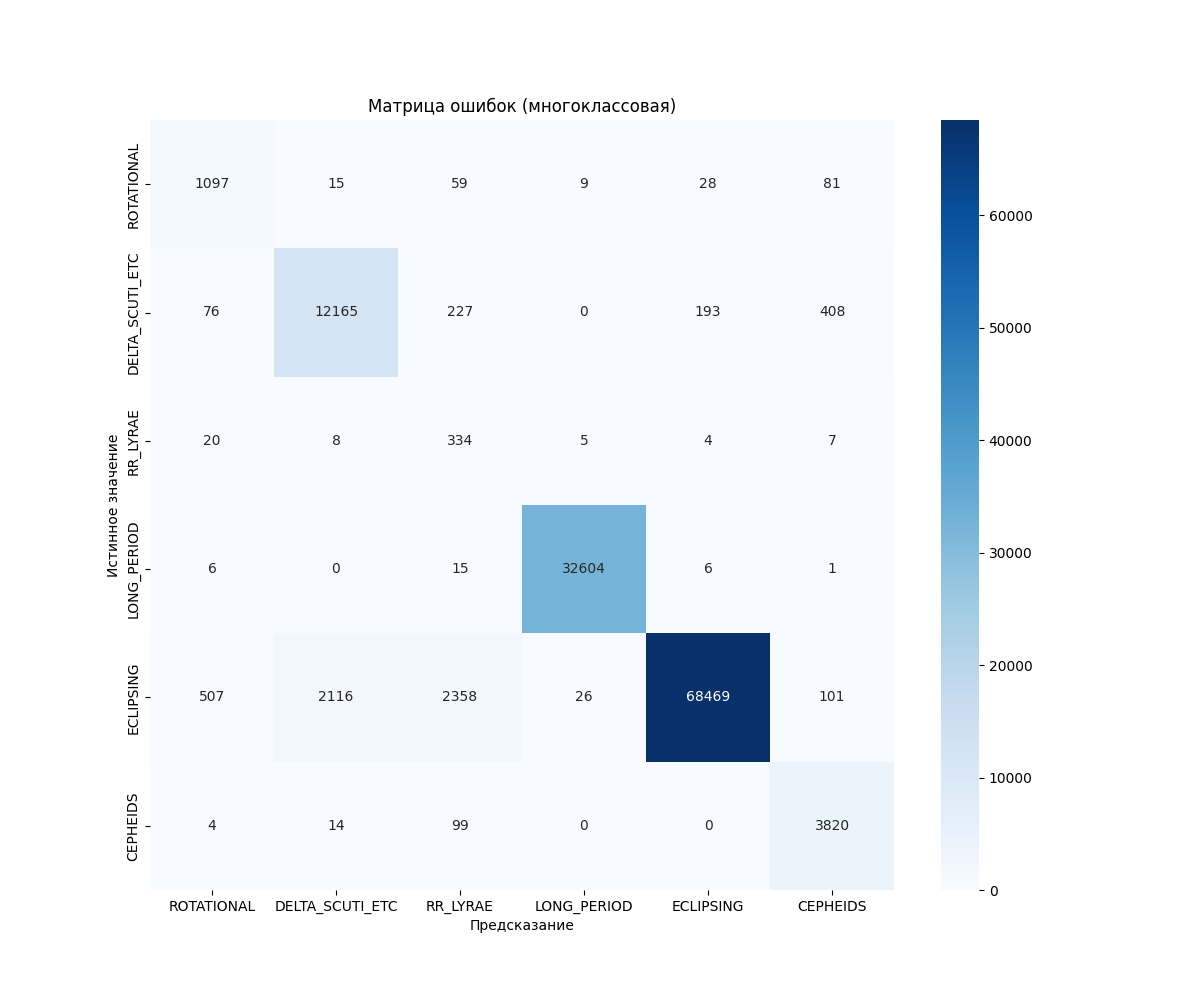
\includegraphics[width=.55\linewidth]{multiclass_confusion_matrix.png}
    \caption{Матрица ошибок мультиклассовой модели.}
    \label{fig:cm-multiclass}
\end{figure}

\subsection{Важность признаков}
Для интерпретации решающего леса, обученного на том же наборе, была построена диаграмма важности (рис.~\ref{fig:feature-imp}). 
На вершине списка ожидаемо оказались цветовые индексы $(G_{\mathrm{BP}}-G_{\mathrm{RP}})$, амплитуда кривой блеска и логарифм периода.

\begin{figure}[H]
    \centering
    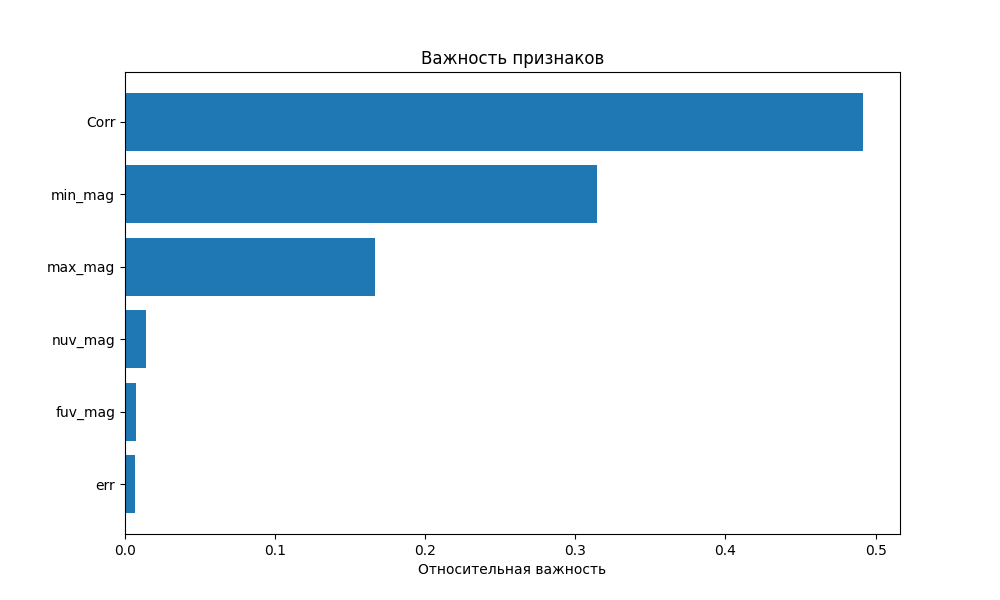
\includegraphics[width=.7\linewidth]{feature_importance.png}
    \caption{Важность признаков по импакт-фактору Gini.}
    \label{fig:feature-imp}
\end{figure}

\section{Выводы и дальнейшие шаги}
\begin{itemize}
    \item Построен бинарный классификатор переменных звёзд с точностью 94~\%. Случайный лес обеспечивает лучший баланс \texttt{precision}/\texttt{recall}.
    \item Создана первичная мультиклассовая модель с суммарной точностью 95~\%. Проблемой остаётся качество на редких и смешанных типах (\texttt{ECLIPSING}).
    \item Дальнейшая работа сосредоточена на:
    \begin{enumerate}
        \item \textbf{расширении тренировочного набора} за счёт каталогов OGLE и ZTF;
        \item \textbf{экстракции временных признаков} (период L-S, амплитуда, статистики формы кривой);
        \item \textbf{переходе к гибридной архитектуре CNN+LSTM}, обрабатывающей фазированные кривые блеска напрямую.
    \end{enumerate}
\end{itemize}

\newpage
\bibliographystyle{unsrt}
\begin{thebibliography}{99}
\bibitem{karachurin2025} Р.~Н.~Карачурин. \textit{Методы машинного обучения для анализа переменных звёзд}. 2025.

\bibitem{Bazin2019} Bazin~et~al. ``Photometric light curves classification with machine learning''. \textit{arXiv preprint}, 2019. URL: \url{https://ar5iv.labs.arxiv.org/html/1909.05032}.

\bibitem{Kim2020} Kim~et~al. ``Variable star classification with machine learning methods''. \textit{Monthly Notices of the Royal Astronomical Society}, 491:3805–3816, 2020. URL: \url{https://academic.oup.com/mnras/article/491/3/3805/5625784}.

\bibitem{Mackenzie2018} Mackenzie~et~al. ``Deep multi-survey classification of variable stars''. \textit{arXiv preprint}, 2018. URL: \url{https://ar5iv.labs.arxiv.org/html/1810.09440}.

\bibitem{Balazs2020} Balázs, Csörgő~et~al. ``Image-based classification of variable stars – First results on OGLE data''. \textit{arXiv preprint}, 2020. URL: \url{https://ar5iv.org/abs/2006.07614}.

\bibitem{Cox1980} Cox, J.~P. ``Stellar Pulsation Theory''. \textit{Annual Review of Astronomy and Astrophysics}, 18:15–42, 1980.

\bibitem{Drake2009} Drake, A.~J.~et~al. ``The Catalina Real-time Transient Survey (CRTS)''. 2009. URL: \url{http://crts.caltech.edu/}.

\bibitem{FreedmanMadore2010} Freedman, W.~L. and B.~F.~Madore. ``The Hubble Constant''. \textit{Annual Review of Astronomy and Astrophysics}, 48:673–710, 2010.

\bibitem{Goodfellow2016} Goodfellow, I., Y.~Bengio and A.~Courville. \textit{Deep Learning}. MIT Press, 2016.

\bibitem{Hilditch2001} Hilditch, R.~W. \textit{An Introduction to Close Binary Stars}. Cambridge University Press, 2001.

\bibitem{Nun2018} Nun, I.~et~al. ``Deep multi-survey classification of variable stars''. \textit{arXiv preprint}, 2018. URL: \url{https://ar5iv.org/abs/1810.09440}.

\bibitem{Nun2020} Nun, I., C.~Mackenzie, J.~Long~et~al. ``Deep multi-survey classification of variable stars''. \textit{Monthly Notices of the Royal Astronomical Society}, 491(3):3805–3816, 2020.

\bibitem{Riess2016} Riess, A.~G.~et~al. ``A 2.4\% Determination of the Local Value of the Hubble Constant''. \textit{The Astrophysical Journal}, 826(1):56, 2016.

\bibitem{Skrutskie2006} Skrutskie, M.~F.~et~al. ``The Two Micron All Sky Survey (2MASS)''. \textit{Astronomical Journal}, 131:1163, 2006.

\bibitem{Wright2010} Wright, E.~L.~et~al. ``The Wide‑field Infrared Survey Explorer (WISE): Mission Description and Initial On‑orbit Performance''. \textit{Astronomical Journal}, 140:1868–1881, 2010.
\end{thebibliography}

\end{document}

\newpage
\bibliographystyle{unsrt}
\begin{thebibliography}{99}
\bibitem{karachurin2025} Р.~Н.~Карачурин. \textit{Методы машинного обучения для анализа переменных звёзд}. 2025.
\bibitem{Bazin2019} Bazin~et~al. ``Photometric light curves classification with machine learning''. \textit{arXiv preprint}, 2019.
\bibitem{Kim2020} Kim~et~al. ``Variable star classification with machine learning methods''. \textit{MNRAS}, 491:3805–3816, 2020.
\bibitem{Mackenzie2018} Mackenzie~et~al. ``Deep multi‑survey classification of variable stars''. \textit{arXiv preprint}, 2018.
\bibitem{Balazs2020} Balázs, Csörgő~et~al. ``Image‑based classification of variable stars – first results on OGLE data''. \textit{arXiv preprint}, 2020.
\bibitem{Cox1980} Cox, J.~P. ``Stellar Pulsation Theory''. \textit{ARA\&A}, 18:15–42, 1980.
\bibitem{Drake2009} Drake, A.~J.~et~al. ``The Catalina Real‑time Transient Survey''. 2009.
\bibitem{FreedmanMadore2010} Freedman, W.~L. and B.~F.~Madore. ``The Hubble Constant''. \textit{ARA\&A}, 48:673–710, 2010.
\bibitem{Goodfellow2016} Goodfellow, I., Y.~Bengio, A.~Courville. \textit{Deep Learning}. MIT Press, 2016.
\bibitem{Hilditch2001} Hilditch, R.~W. \textit{An Introduction to Close Binary Stars}. CUP, 2001.
\bibitem{Nun2018} Nun, I.~et~al. ``Deep multi‑survey classification of variable stars''. \textit{arXiv preprint}, 2018.
\bibitem{Riess2016} Riess, A.~G.~et~al. ``A 2.4\% Determination of the Local Value of the Hubble Constant''. \textit{ApJ}, 826:56, 2016.
\bibitem{Skrutskie2006} Skrutskie, M.~F.~et~al. ``The Two Micron All Sky Survey (2MASS)''. \textit{AJ}, 131:1163, 2006.
\bibitem{Wright2010} Wright, E.~L.~et~al. ``The Wide‑field Infrared Survey Explorer (WISE): Mission Description and Initial On‑orbit Performance''. \textit{AJ}, 140:1868–1881, 2010.
\end{thebibliography}

\end{document}
"""

with open('/mnt/data/report_final.tex', 'w', encoding='utf-8') as f:
    f.write(corrected_tex)
print("Corrected LaTeX saved to /mnt/data/report_final.tex")

